\Class{Barbarian}
{Gith's blood! I will hunt that wizard down and skin him alive.}{Borac, mul barbarian}

Brutality is a way of life in Athas, as much in some of the cities as in the dwindling tribes of Athas' harsh wastes. Cannibal headhunting halflings (who occasionally visit Urik from the Forest Ridge) sometimes express shock at the savagery and bloodshed of the folk that call themselves ``civilized'' and live between walls of stone. They would be more horrified if they were to see the skull piles of Draj, experience the Red Moon Hunt in Gulg, or watch a seemingly docile house slave in Eldaarich rage as she finally ``goes feral'', taking every frustration of her short cruel life out on whoever happens to be closest to hand. Nibenese sages claim that the potential for savagery is in every sentient race, and the history of Athas seems to support their claim.

Some on Athas have turned their brutality into an art of war. They are known as ``brutes'', ``barbarians'' or ``feral warriors'' and they wear the name with pride. Impious but superstitious, cunning and merciless, fearless and persistent, they have carved a name for their martial traditions out of fear and blood.

\WarriorTable{The Barbarian}{
1  & +1             & +2  & +0 & +0 & Fast movement, rage 1/day               \\
2  & +2             & +3  & +0 & +0 & Uncanny dodge                           \\
3  & +3             & +3  & +1 & +1 & Wasteland trap sense +1                 \\
4  & +4             & +4  & +1 & +1 & Rage 2/day                              \\
5  & +5             & +4  & +1 & +1 & Improved uncanny dodge                  \\
6  & +6/+1          & +5  & +2 & +2 & Wasteland trap sense +2                 \\
7  & +7/+2          & +5  & +2 & +2 & Damage reduction 1/--                   \\
8  & +8/+3          & +6  & +2 & +2 & Bonus feat, rage 3/day                  \\
9  & +9/+4          & +6  & +3 & +3 & Greater rage, wasteland trap sense +3   \\
10 & +10/+5         & +7  & +3 & +3 & Damage reduction 2/--                   \\
11 & +11/+6/+1      & +7  & +3 & +3 & Bonus feat                              \\
12 & +12/+7/+2      & +8  & +4 & +4 & Rage 4/day, wasteland trap sense +4     \\
13 & +13/+8/+3      & +8  & +4 & +4 & Indomitable will, damage reduction 3/-- \\
14 & +14/+9/+4      & +9  & +4 & +4 & Bonus feat                              \\
15 & +15/+10/+5     & +9  & +5 & +5 & Tireless rage, wasteland trap sense +5  \\
16 & +16/+11/+6/+1  & +10 & +5 & +5 & Damage reduction 4/--, rage 5/day       \\
17 & +17/+12/+7/+2  & +10 & +5 & +5 & Bonus feat, mighty rage                 \\
18 & +18/+13/+8/+3  & +11 & +6 & +6 & Wasteland trap sense +6                 \\
19 & +19/+14/+9/+4  & +11 & +6 & +6 & Damage reduction 5/--                   \\
20 & +20/+15/+10/+5 & +12 & +6 & +6 & Bonus feat, rage 6/day                  \\
}

\begin{figure}[t!]
\centering
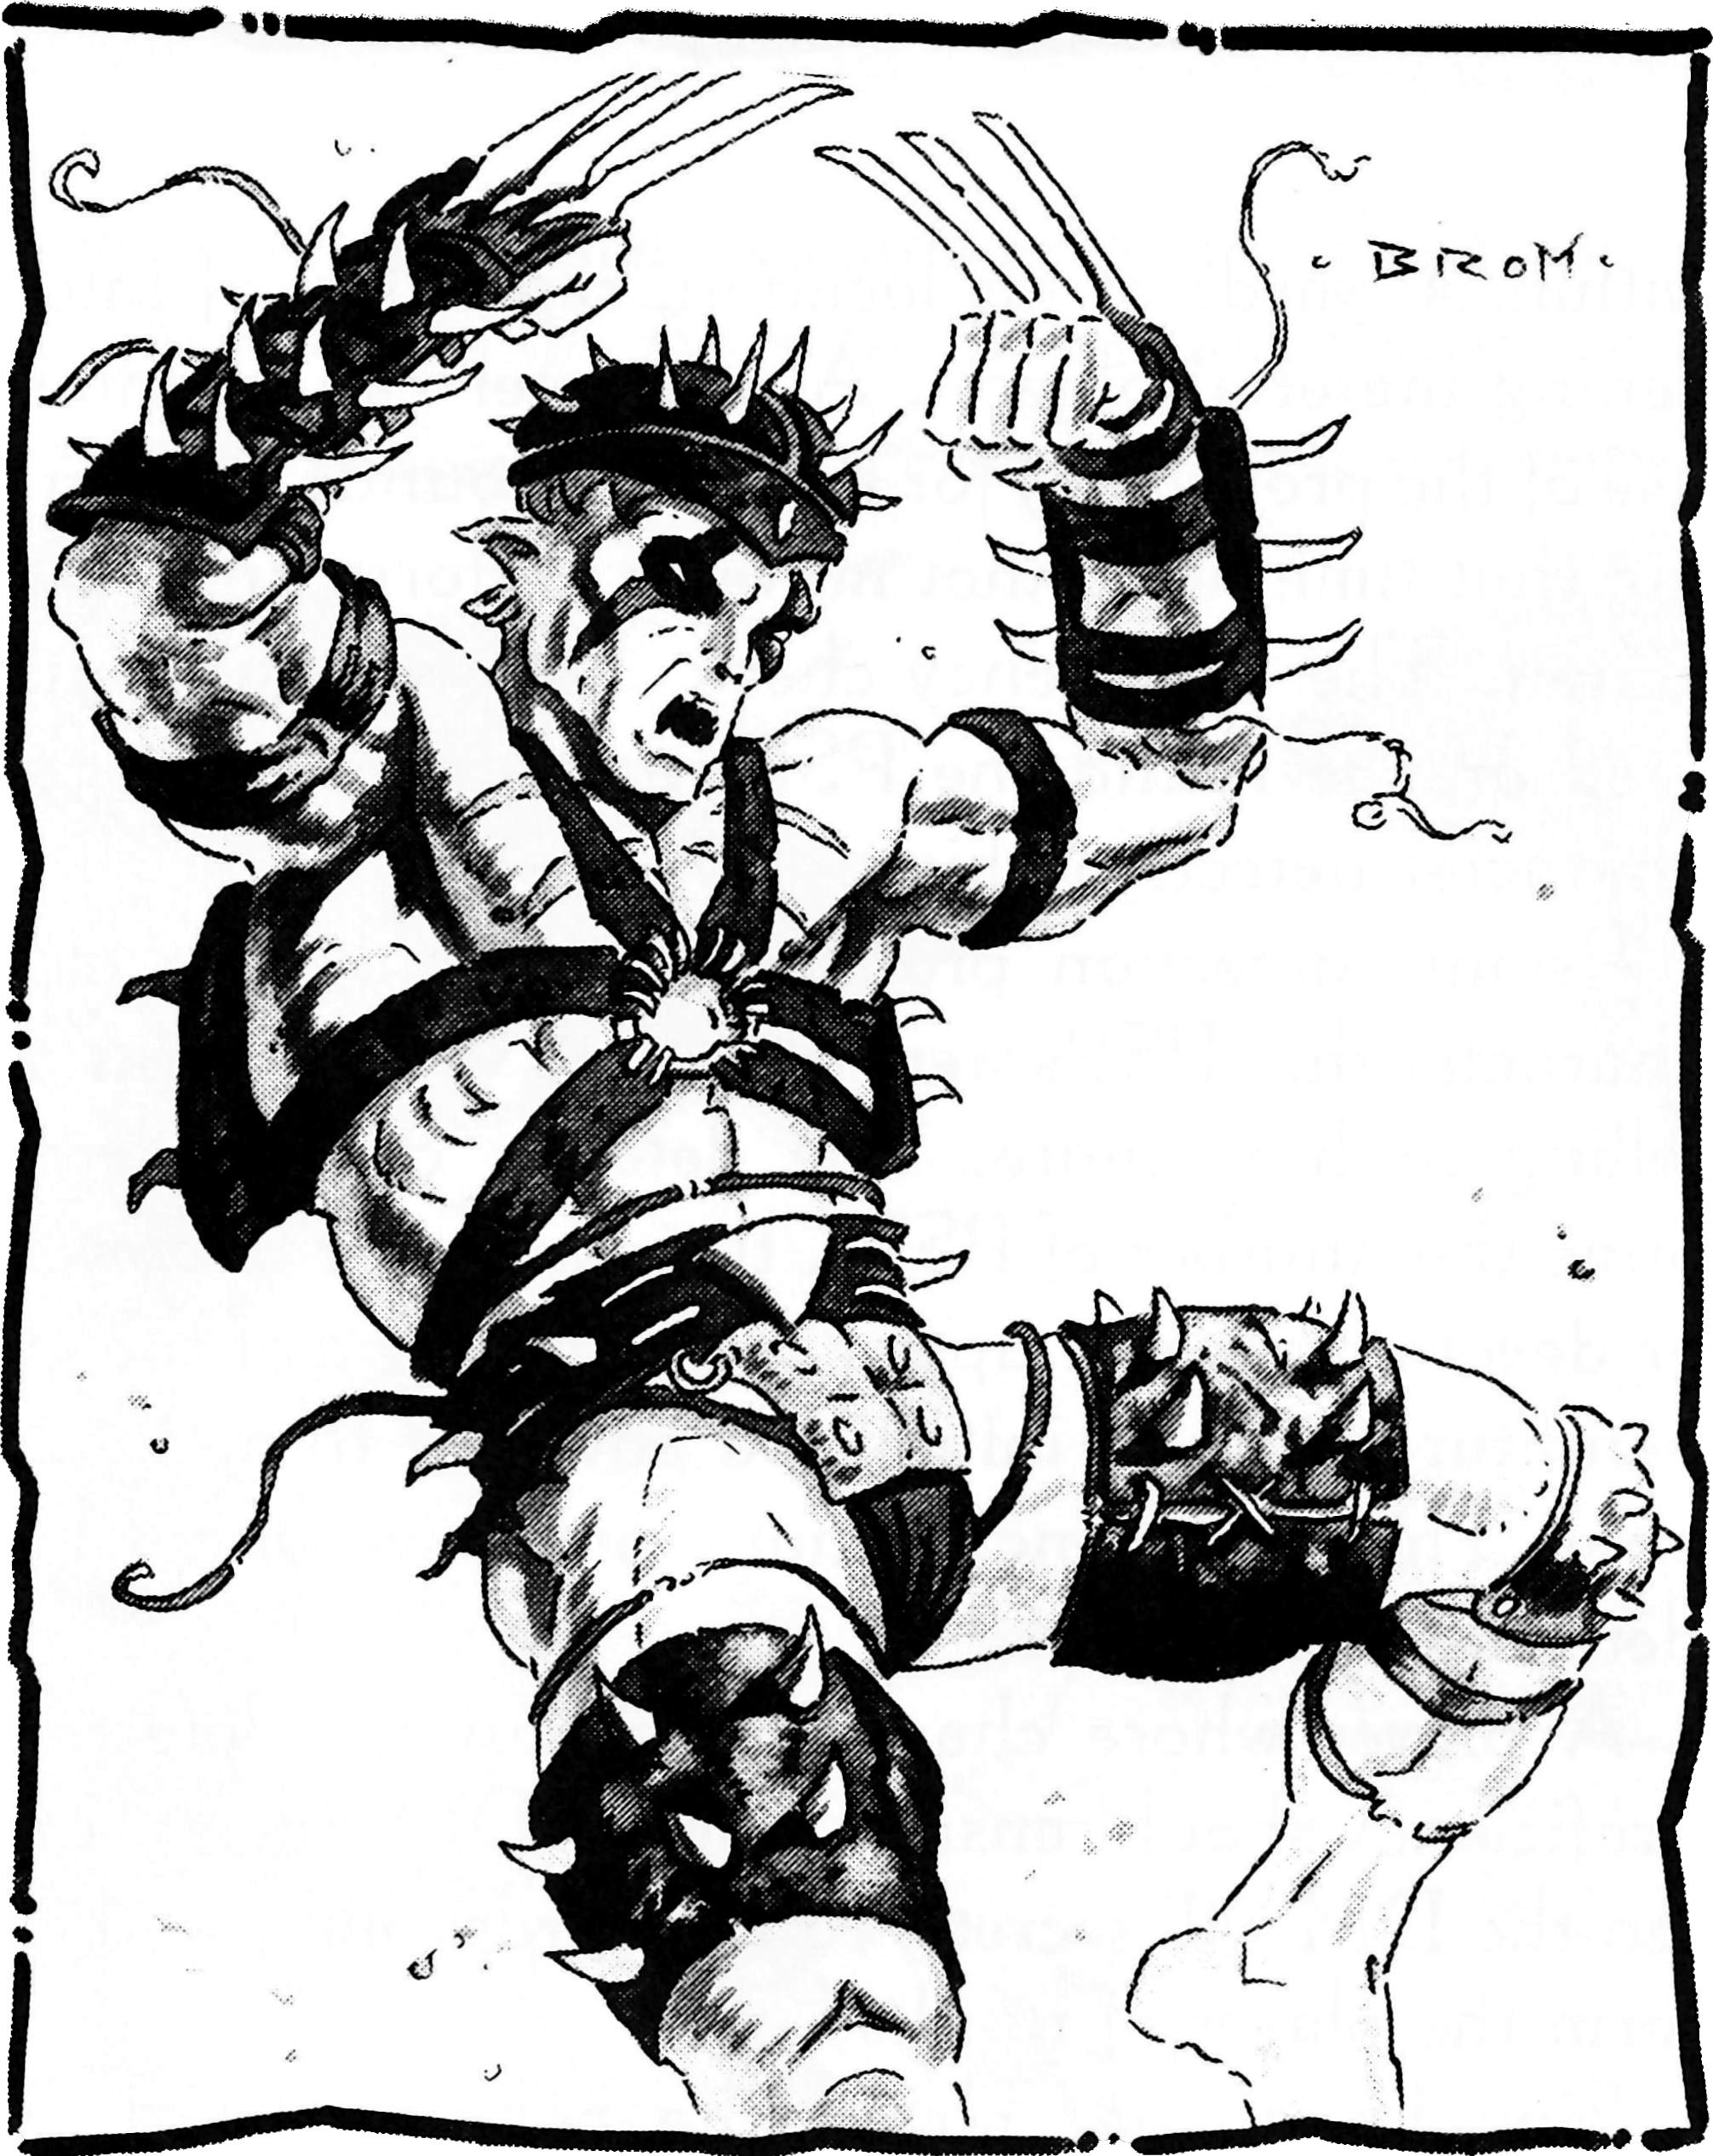
\includegraphics[width=\columnwidth]{images/barbarian-1.png}
\WOTC
\end{figure}

\subsection{Making a Barbarian}

The barbarian is a fearsome warrior, compensating for lack of training and discipline with bouts of powerful rage. While in this berserk fury, barbarians become stronger and tougher, better able to defeat their foes and withstand attacks. These rages leave barbarians winded; at first they only have the energy for a few such spectacular displays per day, but those few rages are usually sufficient.

\textbf{Races:} Humans are often barbarians, many having been raised in the wastes or escaped from slavery. Half-elves sometimes become barbarians, having been abandoned by their elven parents to the desert to survive on their own; if more of them survived they would be quite numerous. Dwarves are very rarely barbarians, but their mul half-children take to brutishness like a bird takes to flight, living by their wits and strengths in the wastes. Muls have a particular inclination this way of life, and very often ``go feral'' in the wilderness after escaping slavery in the city. Elves rarely take to the barbarian class; those that do are usually from raiding tribes such as the Silt Stalkers. Half-giants readily take the barbarian class. Despite their feral reputations, halflings rarely become barbarians; their small statures and weak strength adapts them better for the ranger class. Likewise, despite their wild nature, thri-kreen are rarely barbarians, since their innate memories allow them to gain more specialized classes such as ranger and psychic warrior without training. Pterrans of the Forest Ridge occasionally become barbarians, but like halflings they more often favor the ranger class.

\textbf{Alignment:} Barbarians are never lawful---their characteristic rage is anything but disciplined and controlled. Many barbarians in the cities are often rejects from the regular army, unable to bear regular discipline or training. Some may be honorable, but at heart they are wild. At best, chaotic barbarians are free and expressive. At worst, they are thoughtlessly destructive.

\subsection{Game Rule Information}
\textbf{Alignment:} Any nonlawful.

\textbf{Hit Die:} d12.

\subsubsection{Class Skills}
\skill{Autohypnosis} (Wis), \skill{Climb} (Str), \skill{Craft} (Int), \skill{Escape Artist} (Des), \skill{Handle Animal} (Cha), \skill{Intimidate} (Cha), \skill{Jump} (Str), \skill{Knowledge} (nature) (Int), \skill{Listen} (Wis), \skill{Profession} (Wis), \skill{Ride} (Dex), and \skill{Survival} (Wis).

\textbf{Skill Points per Level:} 4 + Int modifier ($\times4$ at 1st level).

\subsubsection{Class Features}

\textbf{Weapon and Armor Proficiency:} A barbarian is proficient with all simple and martial weapons, light armor, medium armor, and shields (except tower shields).

\textbf{Fast Movement (Ex):} A barbarian's land speed is faster than the norm for his race by +3 meters. This benefit applies only when he is wearing no armor, light armor, or medium armor and not carrying a heavy load. Apply this bonus before modifying the barbarian's speed because of any load carried or armor worn.

\textbf{Rage (Ex):} A barbarian can fly into a rage a certain number of times per day. In a rage, a barbarian temporarily gains a +4 bonus to Strength, a +4 bonus to Constitution, and a +2 morale bonus on Will saves, but he takes a $-2$ penalty to Armor Class. The increase in Constitution increases the barbarian's hit points by 2 points per level, but these hit points go away at the end of the rage when his Constitution  score drops back to normal. (These extra hit points are not lost first the way temporary hit points are.) While raging, a barbarian cannot use any Charisma-, Dexterity-, or Intelligence-based skills (except for \skill{Balance}, \skill{Escape Artist}, \skill{Intimidate}, and \skill{Ride}), the \skill{Concentration} skill, or any abilities that require patience or concentration, nor can he cast spells or activate magic items that require a command word, a spell trigger (such as a wand), or spell completion (such as a scroll) to function. He can use any feat he has except \feat{Combat Expertise}, item creation feats, and metamagic feats. A fit of rage lasts for a number of rounds equal to 3 + the character's (newly improved) Constitution modifier. A barbarian may prematurely end his rage. At the end of the rage, the barbarian loses the rage modifiers and restrictions and becomes fatigued ($-2$ penalty to Strength, $-2$ penalty to Dexterity, can't charge or run) for the duration of the current encounter (unless he is a 15th-level barbarian, at which point this limitation no longer applies).

A barbarian can fly into a rage only once per encounter. At 1st level he can use his rage ability once per day. At 4th level and every four levels thereafter, he can use it one additional time per day (to a maximum of six times per day at 20th level). Entering a rage takes no time itself, but a barbarian can do it only during his action, not in response to someone else's action. 

\textbf{Uncanny Dodge (Ex):} At 2nd level, a barbarian retains his Dexterity bonus to AC (if any) even if he is caught flat-footed or struck by an invisible attacker. However, he still loses his Dexterity bonus to AC if immobilized. If a barbarian already has uncanny dodge from a different class, he automatically gains improved uncanny dodge instead.

\textbf{Wasteland Trap Sense (Ex):} Starting at 3rd level, a barbarian gains a +1 bonus on Reflex saves made to avoid traps and natural hazards, and a +1 dodge bonus to AC against attacks made by traps and natural hazards. These bonuses rise by +1 every three barbarian levels thereafter (6th, 9th, 12th, 15th, and 18th level). Trap sense bonuses gained from multiple classes stack.

\textbf{Improved Uncanny Dodge (Ex):} At 5th level and higher, a barbarian can no longer be flanked. This defense denies a rogue the ability to sneak attack the barbarian by flanking him, unless the attacker has at least four more rogue levels than the target has barbarian levels. If a character already has uncanny dodge from a second class, the character automatically gains improved uncanny dodge instead, and the levels from the classes that grant uncanny dodge stack to determine the minimum level a rogue must be to flank the character.

\textbf{Damage Reduction (Ex):} At 7th level, a barbarian gains Damage Reduction. Subtract 1 from the damage the barbarian takes each time he is dealt damage from a weapon or a natural attack. At 10th level, and every three barbarian levels thereafter (13th, 16th, and 19th level), this damage reduction rises by 1 point. Damage reduction can reduce damage to 0 but not below 0.

\textbf{Bonus Feat:} At 8th level and every three levels thereafter (11th, 14th, 17th, and 20th level), a barbarian gains a bonus feat, which must be selected from the following list:
\feat{Awesome Blow},
\feat{Blind-Fight},
\feat{Cleave},
\feat{Closed Mind},
% \feat{Combat Reflexes},
Destructive Rage\textsuperscript{CW},
\feat{Diehard},
\feat{Endurance},
Extend Rage\textsuperscript{CW},
Extra Rage\textsuperscript{CW},
% Faster Healing\textsuperscript{CW},
Fleet of Foot\textsuperscript{CW},
\feat{Great Cleave},
% \feat{Greater Critical},
Greater Resiliency\textsuperscript{CW},
\feat{Hard as Rock},
\feat{Hostile Mind},
\feat{Improved Bull Rush},
% \feat{Improved Critical},
% \feat{Improved Initiative},
\feat{Improved Sunder},
\feat{Innate Hunter},
Instantaneous Rage\textsuperscript{CW},
Intimidating Rage\textsuperscript{CW},
\feat{Mind Over Body},
\feat{Power Attack},
% \feat{Psionic Hole},
% \feat{Quick Draw},
\feat{Rapid Metabolism},
\feat{Reckless Offense},
\feat{Run},
Steadfast Determination\textsuperscript{PH2},
\feat{Toughness},
\feat{Track},
\feat{Wastelander}.
He must meet all the prerequisites for the feat.

\textbf{Greater Rage (Ex):} At 8th level, a barbarian's bonuses to Strength and Constitution during his rage each increase to +6, and his morale bonus on Will saves increases to +3. The penalty to AC remains at $-2$.

\textbf{Indomitable Will (Ex):} While in a rage, a barbarian of 13th level or higher gains a +4 bonus on Will saves to resist enchantment spells and telepathy powers. This bonus stacks with all other modifiers, including the morale bonus on Will saves he also receives during his rage.

\textbf{Tireless Rage (Ex):} At 15th level and higher, a barbarian no longer becomes fatigued at the end of his rage.

\textbf{Mighty Rage (Ex):} At 17th level, a barbarian's bonuses to Strength and Constitution during his rage each increase to +8, and his morale bonus on Will saves increases to +4. The penalty to AC remains at $-2$.

\subsubsection{Ex-Barbarians}

A barbarian who becomes lawful loses the ability to rage and cannot gain more levels as a barbarian. He retains all the other benefits of the class (damage reduction, fast movement, wasteland trap sense, and uncanny dodge).

\subsection{Playing a Barbarian}

All cower and stand in awe at the fury you can tap, enhancing your strength and toughness. But what do these people know of the burnt wastes of Athas, the hellish jungles of the Forest Ridge? The cruel vicissitudes of growing up in the wastes of Athas were nothing but normal to you. When your family was lost in a tembo attack, or when your entire village was either murdered or forced into slavery, how could you not know they might not had to die? These and many other brutal experiences marked you, and you now stand apart from those born into the ``comforts'' of the city-states.

% \vskip5cm
\subsubsection{Religion}

Although most are profoundly superstitious, barbarians distrust the established elemental temples of the cities. Some worship the elements of fire or air or devote themselves to a famous figure. Most barbarians truly believe the sorcerer-kings to be gods, because of their undeniable power, and a few actually worship a sorcerer-king, usually the one that conquered their tribe. Such barbarians often escape menial slavery by joining an elite unit of barbarians in the service of an aggressive city-state such as Urik, Draj or Gulg.

\subsubsection{Other Classes}

Barbarians are most comfortable in the company of gladiators, and of clerics of Air and Fire. Enthusiastic lovers of music and dance, barbarians admire bardic talent, and some barbarians also express fascination with bardic poisons, antidotes and alchemical concoctions. With some justification, barbarians do not trust wizardry. Even though many barbarians manifest a wild talent, they tend to be wary of psions and Tarandan psionicists. Psychic warriors, on the other hand, are creatures after the barbarian's own heart, loving battle for its own sake. Barbarians have no special attitudes toward fighters or rogues. Barbarians admire gladiators and will ask about their tattoos and exploits, but will quickly grow bored if the gladiator does not respond boastfully.

\subsubsection{Combat}

You know that half the battle occurs before the fight even begins. You prefer to choose your battleground when you can, stalking your opponent into terrain that best suits your abilities. Once battle is joined, you become a wild frenzy of motion, striking quickly and powerfully until all your opponents are crushed. While you lack the training of the fighter, or the cunning of the gladiator, you more than compensate them through sheer power and resilience.

\subsubsection{Advancement}

Becoming a barbarian let you further tap into your feral nature, letting you become one with the savage beast in your hear, and through your training, you have learned what you must do to unlock it.

To fully utilize your barbarian abilities, you will want to focus on feats that take advantage of your superior strength and speed, such as Power Attack and Whirlwind Attack.

% \clearpage
\subsection{Starting Packages}
\subsubsection{The Survivor}
Human Barbarian

\textbf{Ability Scores:} Str 15, Dex 13, Con 14, Int 10, Wis 12, Cha 8.

\textbf{Skills:} \skill{Climb}, \skill{Escape Artist}, \skill{Listen}, \skill{Survival}.

\textbf{Languages:} Common.

\textbf{Feat:} \feat{Great Fortitude}, \feat{Wastelander}.

\textbf{Weapons:} Carrikal (1d8/$\times$3)

Atlatl with 10 javelins (1d6/$\times$3, 12 m).

\textbf{Armor:} Scale mail (+4 AC).

\textbf{Gear:} Standard adventurer's kit, 13 cp.

\subsubsection{The Crusher}
Half-giant Barbarian

\textbf{Ability Scores:} Str 23, Dex 10, Con 18, Int 6, Wis 9, Cha 4.

\textbf{Skills:} \skill{Climb}, \skill{Intimidate}, \skill{Jump}.

\textbf{Languages:} Common.

\textbf{Feat:} \feat{Exotic Weapon Proficiency} (swatter).

\textbf{Weapons:} Swatter (3d8/$\times$4).

\textbf{Armor:} Leather (+2 AC).

\textbf{Gear:} Standard adventurer's kit, 0 cp.

\subsubsection{The Hunter}
Thri-kreen Barbarian

\textbf{Ability Scores:} Str 15, Dex 14, Con 12, Int 10, Wis 13, Cha 8.

\textbf{Skills:} \skill{Jump}, \skill{Knowledge} (nature), \skill{Search}, \skill{Survival}.

\textbf{Languages:} Kreen.

\textbf{Feat:} \feat{Track}.

\textbf{Weapons:} Four chatkchas (1d6, 6 m).

\textbf{Armor:} Heavy wooden shield (+2 AC).

\textbf{Gear:} Standard adventurer's kit, 13 cp.

\subsection{Barbarians on Athas}
\Quote{Don't make my friend angry. You won't like him when he's angry.}{Cabal, half-elven bard}

In a savage world like Athas, is only natural that some of its inhabitants have turned into barbarians. They are fierce combatants without the army training fighters receive or wild rangers without the hunting skills.

\subsubsection{Daily Life}

A barbarian is a passionate adventurer. As a survivalist, he often sees his involvement in a particular enterprise as a validation of his superior strength and resilience. In his mind, his presence alone is enough to ensure the success of a quest, adventure, or ruin raid. Even simple tasks are additional opportunities to prove his own worth by accomplishing the task with might and alacrity. Barbarians are typically hardheaded and unforgiving because of the rigors of his previous life.

\subsubsection{Notables}

It is rare for a barbarian to live long enough, or close enough to civilization, in order to become famous, but a few examples exist. Korno, a Raamite gladiator, became the leader of a group of slaves, and Korno's furious rage known from the arenas has only increased after losing everything in the Raam invasion by Dregoth. The leader of Pillage, Chilod, is a tarek know for his outbursts of rage and cruelty, being one of the most feared chiefs of the Bandit States.

\subsubsection{Organizations}

Because of their independent and sometimes downright chaotic natures, many barbarians refuse to join organizations of any kind, though they usually maintain relationships with trading houses and raiding tribes. There is no specific organization that binds barbarians together.

\subsubsection{NPC Reactions}

Many lay people cannot tell a barbarian from a ranger or a fighter until his rage overcomes him and he starts screaming and bashing. Most authority figures and templars do not appreciate barbarians since they are prone to losing control and cannot be truly trusted. Thus, they generally treat barbarians with a great deal of caution.

\subsubsection{Barbarian Lore}

Characters with ranks in \skill{Knowledge} (nature) can research barbarians to learn more about them. When a character makes a skill check, read or paraphrase the following, including the information from lower DCs.

\textbf{DC 10:} Barbarians are hot-blooded combatants who fight with great brutality and savagery.

\textbf{DC 15:} Barbarians become stronger and more resilient when they lose control.

\textbf{DC 20:} Barbarians can stand up to punishment that no other individual can endure, and their reflexes are as quick as a rogue's.